\section{Künstliche Neuronale Netze}%
\label{sec:ann}

\begin{frame}{Künstliches Neuron}
  \begin{minipage}{.65\textwidth}
    \begin{tikzpicture}[->, >=stealth, thick, scale=.8]
      \node [circle split,draw,rotate=90] (z) at (0, 0) {\rotatebox{-90}{$\displaystyle\sum$} \nodepart{lower} \rotatebox{-90}{$\sigma(z)$}};
      \foreach \i in {5,...,1} {
        \node (x-\i) at (-7, 4.5+1.5*-\i) {\(x_{\i}\)};
        \path (x-\i) edge node[above] {\(w_{\i}\)} (z);
      }
      \node (y) at (4, 0) {\(a\)};
      \path (z) edge (y);
      \node (b) at (0, 2.5) {\(b\)};
      \draw (b) -- (z);
    \end{tikzpicture}
  \end{minipage}%
  \begin{minipage}{.35\textwidth}
    \uncover<2->{
      \begin{flushright}
        \begin{tabular}{cl}
          \toprule
          \(\mathbf{x}\)  & Inputvektor\\
          \(\mathbf{w}\)  & Gewichtsvektor\\
          \(b\)  & Bias\\
          \(z\)  & Zwischensumme \(\left(\sum\right)\)\\
          \(\sigma(x)\)  & Aktivierungsfunktion\\
          \(a\)  & Aktivierung/ Output\\
          \bottomrule
        \end{tabular}
      \end{flushright}
    }
  \end{minipage}

  \only<3>{
    \[z = \sum_{i}x_{i}w_i + b = \mathbf{xw} + b\]

    {\centering\(\Rightarrow z\) wird für spätere Parameteroptimierung benötigt\par}
  }
\end{frame}

\begin{frame}{Aktivierungsfunktion \(\sigma(x)\)}
  \begin{minipage}{.45\textwidth}
    \(\Rightarrow\) Es gibt eine Vielzahl verschiedener Aktivierungsfunktionen für unterschiedliche Problemstellungen, für uns soll jedoch lediglich die \textbf{Sigmoid-Funktion} relevant sein:

    \vspace{1cm}

    \[\sigma(x) = \frac{1}{1 + e^{-x}}\]
  \end{minipage}\hfill%
  \begin{minipage}{.5\textwidth}
    \only<2>{
      \begin{tikzpicture}
        \begin{axis}[width=\textwidth, mlineplot, samples=50, ymin=-.1, ymax=1.1, domain=-10:10, title=Sigmoid-Funktion, xlabel=\(x\), ylabel=\(\sigma(x)\)]
          \addplot{1/(1+exp(-x))};
        \end{axis}
      \end{tikzpicture}
    }
  \end{minipage}

\end{frame}

\begin{frame}{Architektur eines Neuronalen Netzwerks}
  \def\layersep{3.5cm}
  \begin{center}
    \alt<2>{
      \begin{tikzpicture}[->, >=stealth, node distance=\layersep]
        \tikzstyle{every pin edge}=[<-,shorten <=1pt]
        \tikzstyle{neuron}=[circle,draw,minimum size=17pt,inner sep=0pt]
        
        % Draw the input layer nodes
        \foreach \y in {1,...,3}
        \node[neuron, pin=left:\(x_{\y}\)] (I-\y) at (0,-\y) {};

        % Draw the nodes for the second hidden layer
        \foreach \y in {1,...,5}
        \path[yshift=(5cm - 3cm)/2] node[neuron] (H1-\y) at (\layersep,-\y cm) {};

        % Draw the output layer nodes
        \foreach \y in {1,...,2}
        \path[yshift=(2cm - 3cm)/2] node[neuron,pin={[pin edge={->}]right:\(y_{\y}\)}] (O-\y) at (2*\layersep,-\y cm) {};

        \foreach \source in {1,...,3}
        \foreach \dest in {1,...,5}
        \path (I-\source) edge (H1-\dest);

        \foreach \source in {1,...,5}
        \foreach \dest in {1,...,2}
        \path (H1-\source) edge (O-\dest);

        \node[above of=H1-1, node distance=1cm] (hidden) {Hidden Layer};
        \node[right of=hidden] (output) {Output Layer};
        \node[left of=hidden] (input) {Input Layer};
      }{
        \begin{tikzpicture}[->, >=stealth]
          \tikzstyle{every pin edge}=[<-,shorten <=1pt]
          \tikzstyle{neuron}=[circle,draw,minimum size=17pt,inner sep=0pt]
          
          % Draw the input layer nodes
          \foreach \y in {1,...,3}
          \node[neuron, pin=left:] (I-\y) at (0,-\y) {};

          % Draw the nodes for the second hidden layer
          \foreach \y in {1,...,5}
          \path[yshift=(5cm - 3cm)/2] node[neuron] (H1-\y) at (\layersep,-\y cm) {};

          % Draw the output layer nodes
          \foreach \y in {1,...,2}
          \path[yshift=(2cm - 3cm)/2] node[neuron,pin={[pin edge={->}]right:}] (O-\y) at (2*\layersep,-\y cm) {};

          \foreach \source in {1,...,3}
          \foreach \dest in {1,...,5}
          \path (I-\source) edge (H1-\dest);

          \foreach \source in {1,...,5}
          \foreach \dest in {1,...,2}
          \path (H1-\source) edge (O-\dest);
        }
      \end{tikzpicture}
    \end{center}
  \end{frame}

  \begin{frame}{Deep Neural Network}
    \begin{center}
      \dnn{5, 6, 5, 7, 3}
    \end{center}
  \end{frame}

  \begin{frame}{Target-Architektur zur Klassifikation von MNIST}
    \def\layersep{2.5cm}
    \begin{center}
      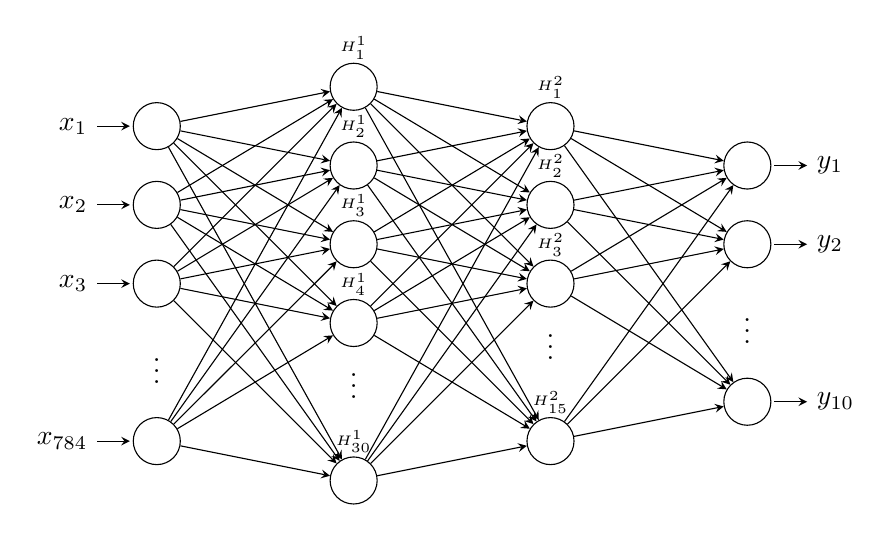
\begin{tikzpicture}[->, >=stealth, node distance=\layersep]
        \tikzstyle{every pin edge}=[<-,shorten <=1pt]
        \tikzstyle{neuron}=[circle,draw,minimum size=17pt,inner sep=0pt]
        
        \node[neuron, pin=left:\(x_{1}\)] (I-1) at (0,-1) {}; \node[neuron,
        pin=left:\(x_{2}\)] (I-2) at (0,-2) {}; \node[neuron,
        pin=left:\(x_{3}\)] (I-3) at (0,-3) {}; \node at (0, -4) {\(\vdots\)};
        \node[neuron, pin=left:\(x_{784}\)] (I-4) at (0,-5) {};

        \path[yshift=(6cm - 5cm)/2] node[neuron] (H1-1) at (\layersep,-1 cm) {};
        \path[yshift=(6cm - 5cm)/2] node[neuron] (H1-2) at (\layersep,-2 cm) {};
        \path[yshift=(6cm - 5cm)/2] node[neuron] (H1-3) at (\layersep,-3 cm) {};
        \path[yshift=(6cm - 5cm)/2] node[neuron] (H1-4) at (\layersep,-4 cm) {};
        \path[yshift=(6cm - 5cm)/2] node at (\layersep, -4.7cm) {$\vdots$};
        \path[yshift=(6cm - 5cm)/2] node[neuron] (H1-5) at (\layersep,-6 cm) {};

        \path node[neuron] (H2-1) at (2*\layersep,-1 cm) {}; \path node[neuron]
        (H2-2) at (2*\layersep,-2 cm) {}; \path node[neuron] (H2-3) at
        (2*\layersep,-3 cm) {}; \path node at (2*\layersep, -3.7cm) {$\vdots$};
        \path node[neuron] (H2-4) at (2*\layersep,-5 cm) {};

        \path[yshift=(2cm - 3cm)/2] node[neuron,pin={[pin
          edge={->}]right:\(y_{1}\)}] (O-1) at (3*\layersep,-1 cm) {};
        \path[yshift=(2cm - 3cm)/2] node[neuron,pin={[pin
          edge={->}]right:\(y_{2}\)}] (O-2) at (3*\layersep,-2 cm) {};
        \path[yshift=(2cm - 3cm)/2] node at (3*\layersep, -3cm) {$\vdots$};
        \path[yshift=(2cm - 3cm)/2] node[neuron,pin={[pin
          edge={->}]right:\(y_{10}\)}] (O-3) at (3*\layersep,-4 cm) {};

        \foreach \source in {1,...,4} \foreach \dest in {1,...,5} \path
        (I-\source) edge (H1-\dest);

        \foreach \source in {1,...,5} \foreach \dest in {1,...,4} \path
        (H1-\source) edge (H2-\dest);

        \foreach \source in {1,...,4} \foreach \dest in {1,...,3} \path
        (H2-\source) edge (O-\dest);

        \foreach \y [count=\i] in {1,2,3,4,30} \node[node distance=14pt, above
        of=H1-\i] {\tiny\(H^1_{\y}\)};

        \foreach \y [count=\i] in {1,2,3,15} \node[node distance=14pt, above
        of=H2-\i] {\tiny\(H^2_{\y}\)};
      \end{tikzpicture}
    \end{center}
  \end{frame}
  
  \begin{frame}{Vektorisierung der Gewichte \(w\) und der Biases \(b\)}
    \def\layersep{2.5cm}
    \begin{tikzpicture}[->, >=stealth, node distance=\layersep, spy using outlines={circle, magnification=5, size=7cm, connect spies}]
      \begin{scope}[scale=.5, transform shape]
        \tikzstyle{every pin edge}=[<-,shorten <=1pt]
        \tikzstyle{neuron}=[circle,draw,minimum size=17pt,inner sep=0pt]

        % Input Neurons
        \node[neuron, pin=left:\(x_{1}\)] (I-1) at (0,-1) {};
        \node[neuron, pin=left:\(x_{2}\)] (I-2) at (0,-2) {};
        \node[neuron, pin=left:\(x_{3}\)] (I-3) at (0,-3) {};
        \node at (0, -4) {\(\vdots\)};
        \node[neuron, pin=left:\(x_{784}\)] (I-4) at (0,-5) {};

        % Neurons in first hidden layer
        \path[yshift=(6cm - 5cm)/2] node[neuron] (H1-1) at (\layersep,-1 cm) {};
        \path[yshift=(6cm - 5cm)/2] node[neuron] (H1-2) at (\layersep,-2 cm) {};
        \path[yshift=(6cm - 5cm)/2] node[neuron] (H1-3) at (\layersep,-3 cm) {};
        \path[yshift=(6cm - 5cm)/2] node[neuron] (H1-4) at (\layersep,-4 cm) {};
        \path[yshift=(6cm - 5cm)/2] node at (\layersep, -4.7cm) {$\vdots$};
        \path[yshift=(6cm - 5cm)/2] node[neuron] (H1-5) at (\layersep,-6 cm) {};

        % Neurons in second hidden layer
        \path node[neuron] (H2-1) at (2*\layersep,-1 cm) {};
        \path node[neuron] (H2-2) at (2*\layersep,-2 cm) {};
        \path node[neuron] (H2-3) at (2*\layersep,-3 cm) {};
        \path node at (2*\layersep, -3.7cm) {$\vdots$};
        \path node[neuron] (H2-4) at (2*\layersep,-5 cm) {};

        % Neurons in output layer
        \path[yshift=(2cm - 3cm)/2] node[neuron,pin={[pin edge={->}]right:\(y_{1}\)}] (O-1) at (3*\layersep,-1 cm) {};
        \path[yshift=(2cm - 3cm)/2] node[neuron,pin={[pin edge={->}]right:\(y_{2}\)}] (O-2) at (3*\layersep,-2 cm) {};
        \path[yshift=(2cm - 3cm)/2] node at (3*\layersep, -3cm) {$\vdots$};
        \path[yshift=(2cm - 3cm)/2] node[neuron,pin={[pin edge={->}]right:\(y_{10}\)}] (O-3) at (3*\layersep,-4 cm) {};

        \foreach \source in {1,...,4}
        \foreach \dest in {1,...,5}
        \path (I-\source) edge (H1-\dest);

        \foreach \source in {1,...,5}
        \foreach \dest in {1,...,4}
        \path (H1-\source) edge (H2-\dest);

        \foreach \source in {1,...,4}
        \foreach \dest in {1,...,3}
        \path (H2-\source) edge (O-\dest);

        \foreach \y [count=\i] in {1,2,3,4,30}
        \node[node distance=14pt, above of=H1-\i] {\tiny\(H^1_{\y}\)};

        \foreach \y [count=\i] in {1,2,3,15}
        \node[node distance=14pt, above of=H2-\i] {\tiny\(H^2_{\y}\)};

        \spy[myblue] on (H1-1) in node (a) at (10, -3.5);
      \end{scope}
      \only<2->{
        \begin{scope}[myorange, yshift=-1.5cm]
          \draw[-, line width=.7mm, black] (10, -1.25cm) -- (10, -2.75cm);
          \node (sum) at (9.65, -2) {\large\(\sum\)};
          \node (act) at (10.4, -2) {\(\sigma(z)\)};
          \node (x1) at (7.8, -2.1) {\small\(x_1w^1_{1,1}\)};
          \node (x2) at (7.6, -3) {\small\(x_2w^1_{1,2}\)};
          \node (x3) at (7.8, -3.65) {\small\(x_3w^1_{1,3}\)};
          \node[fill=white] (x4) at (9, -3.8) {\small\(x_{784}w^1_{1,784}\)};
          \node (a1) at (12, -2.15) {\small\(a^1_1\)};
          \node (a2) at (11.8, -2.8) {\small\(a^1_1\)};
          \node (a3) at (11.6, -3.3) {\small\(a^1_1\)};
          \node (a4) at (11.05, -3.4) {\small\(a^1_1\)};
        \end{scope}
      }
      \uncover<3->{
        \node at (2.5, -5) {\footnotesize\(\displaystyle \mathbf{W^1} =
          \begin{bmatrix}
            w^1_{1,1} & w^1_{2,1} & \cdots & w^1_{30,1}\\
            w^1_{1,2} & w^1_{2,2} & \cdots & w^1_{30,2}\\
            \vdots & \vdots & \ddots & \vdots\\
            w^1_{1,784} & w^1_{2,784} & \cdots & w^1_{30,784}
          \end{bmatrix};~
          \mathbf{b^1} =
          \begin{bmatrix}
            b^1_1\\b^1_2\\\vdots\\b^1_{30}
          \end{bmatrix}
          \)};
      }
    \end{tikzpicture}
  \end{frame}


  %%% Local Variables:
  %%% mode: latex
  %%% TeX-master: "../präsentation"
  %%% End:
